\subsection{Term Structure and Interest Rate Dynamics}

\begin{definition} \hlt{Spot Curve (Zero Curve, Strip Curve)}\\
The yield-to-maturity of a series of default-risk-free zero-coupon bonds, for a full range of maturities.\\
The yield-to-maturity is stated on a semi-annual basis.
\end{definition}

\begin{figure}[H]
\centering
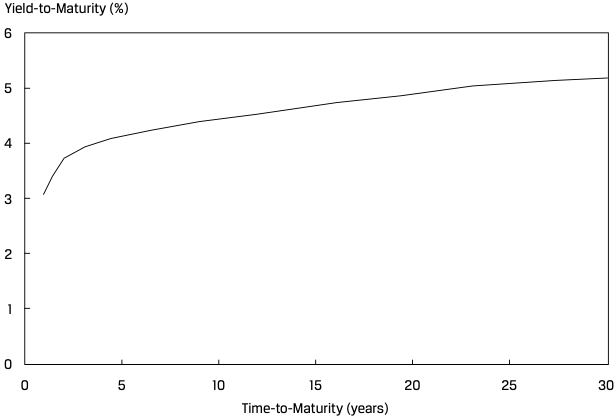
\includegraphics[scale=0.4]{/fi/spotcurve}
\caption{Government Bond Spot (Zero) Curve}
\end{figure}

\begin{definition} \hlt{Yield Curve}\\
Only the most recently-issued and actively traded government bonds are used to build the yield curve.\\
This is constructed on the basis of observed yields and maturities. Points are connected with linear interpolation.\\
Curve also include money market (non-coupon-bearing) bonds, converted to bond equivalent yields.
\end{definition}

\begin{figure}[H]
\centering
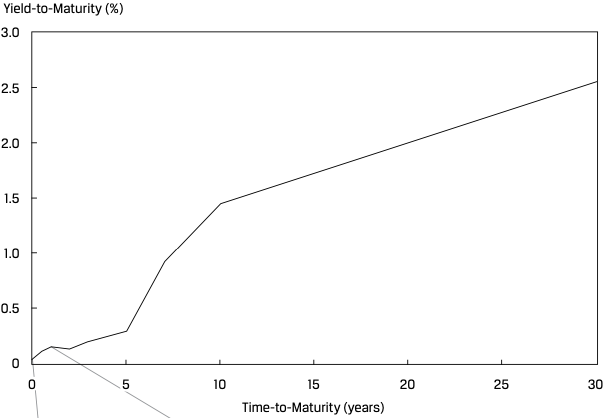
\includegraphics[scale=0.4]{/fi/yieldcurve}
\caption{Government Bond Yield Curve}
\end{figure}

\begin{method} \hlt{Bond Pricing with Spot Rates}\\
Given a sequence of spot rates, the bond price would be
\begin{equation}
PV = \sum\limits_{t=1}^N \frac{PMT}{(1+Z_t)^t} + \frac{FV}{(1+Z_N)^N} \nonumber
\end{equation}
where $Z_t$ is the spot rate, or zero-coupon yield, or zero rate, for period $t$.\\
For pricing a bond with different risk profile than the spot curve, a spread will be added to spot rates.
\end{method}

\begin{method} \hlt{Par Rate}\\
A yield-to-maturity that makes the present value of a bond’s cash flows equal to par.\\
Solve for $PMT$ given a sequence of spot rates $Z_t$. Between coupon dates, set the flat price to $100$.\\
Par rate is then $PMT/100$.
\begin{equation}
100 = \sum\limits_{t=1}^N \frac{PMT}{(1+Z_t)^t} + \frac{PMT}{(1+Z_N)^N} \nonumber
\end{equation}
\end{method}

\begin{method} \hlt{Implied Forward Rates (Forward Yields)}\\
Breakeven reinvestment rates. The rates link the return on an investment in a shorter-term zero-coupon bond to the return on an investment in a longer-term zero-coupon bond.\\
The naming convention is $AyBy$, where $A$ refers to length of forward period in years from today, $B$ is tenor of the bond or its remaining time-to-maturity.\\
The implied forward rate $IFR_{A, B-A}$ begins at $t=A$ and matures at $t=B$, with tenor $B-A$.
\begin{equation}
(1+Z_A)^A \times (1+IFR_{A, B-A})^{B-A} = (1+Z_B)^B \nonumber
\end{equation}\\
Forward curve is a series of forward rates with same tenor but different beginning time.\\
\end{method}

\begin{figure}[H]
\centering
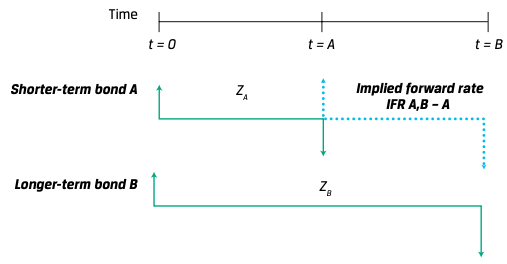
\includegraphics[scale=0.5]{/fi/ifr}
\caption{Implied Forward Rates}
\end{figure}

\begin{method} \hlt{Forward Rate Model}\\
The forward rate model relates forward and spot rates.
\begin{align}
1 + F_{A, B-A} &= \left[ \frac{1+Z_B}{1+Z_A} \right]^{\frac{A}{B-A}} (1+Z_B) \nonumber
\end{align}
\end{method}

\begin{method} \hlt{Spot Rate and Forward Rate Relationship}\\
Spot curve is calculated as a geometric average of forward rates.
\begin{align}
Z_T &= \left[(1+Z_1)\prod\limits_{t=1}^{T-1} (1+F_{t,1}) \right]^{\frac{1}{T}} - 1 \nonumber
\end{align}
\end{method}

\begin{figure}[H]
\centering
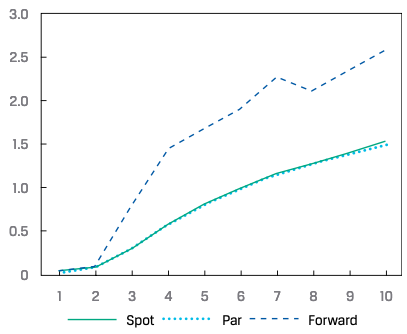
\includegraphics[scale=0.35]{/fi/normalcurve}\hfill
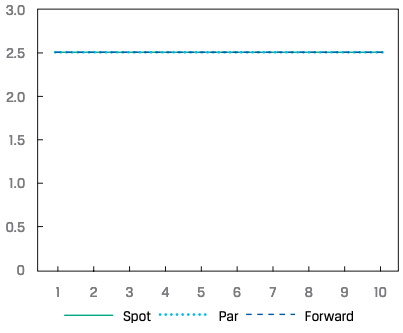
\includegraphics[scale=0.35]{/fi/flatcurve}\hfill
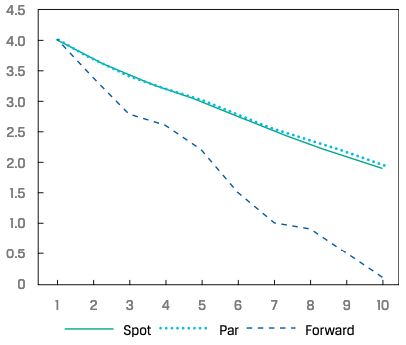
\includegraphics[scale=0.35]{/fi/invertedcurve}
\caption{Upward sloping curve, flat curve, inverted curve}
\end{figure}

\begin{flushleft}
Spot, Par, Forward Curve Relationship
\begin{tabularx}{\textwidth}{X|X|X}
\hline
\rowcolor{gray!30}
Spot Curve Shape & Par Curve & Forward Curve \\
\hline
Upward Sloping & Below Spot Curve & Above Spot Curve \\
\hline
Flat & Equal to Spot Curve & Equal to Spot Curve \\
\hline
Inverted & Above Spot Curve & Below Spot Curve \\
\hline
\end{tabularx}
\end{flushleft}

\begin{definition} \hlt{Discount Factor}\\
Price of a $\$1$ par zero-coupon bond after $N$ periods, denoted $PV_N$.\\
The $N$-period discount factor (denoted $DF_N$) is the discount function.
\begin{equation}
DF_N = \frac{1}{(1+Z_N)^N} \nonumber
\end{equation}
where $Z_N$ is the spot rate at time $N$.\\
In relation to forward rate $F_{A, B-A}$, given the forward contract price $DF_{A, B-A}$,
\begin{equation}
DF_{A, B-A} = \frac{1}{\left(1 + F_{A, B-A} \right)^{B-A}} \nonumber
\end{equation}
\end{definition}

\begin{method} \hlt{Bootstrapping}\\
Process considers a coupon-paying bond as a portfolio of zero-coupon bonds.\\
The zero-coupon rates are determined by using  par yields and solving for zero-coupon rates one-by-one, from shortest to longest maturities, using a forward substitution process.
\end{method}

\begin{definition} \hlt{Swap Rate Curve}\\
Curve based on the fixed rate of an interest rate swap. The swap rate is derived using short-term lending rates rather than default risk-free rates (as seen in YTM on government bonds).\\
The swap rate curve is derived from varying fixed rate component of swap rates for different maturities.
\end{definition}

\begin{remark} \hlt{Preference of Using Swap Rates for Valuing Bonds}\\
Swap rate curve is used as benchmark interest rate curve rather than government bond yield curve as:
\begin{enumerate}[label=\roman*.]
\setlength{\itemsep}{0pt}
\item swap rates reflect credit risk of commercial banks rather than that of governments
\item swap market is not regulated by government, which makes swap rates in different countries more comparable. Government bond yield curves reflect sovereign risk unique in each country.
\item swap curve has yield quotes at many maturities, while government bond yield curve has on-the-run issues trading at only a small number of maturities.
\end{enumerate}
Wholesale banks that manage interest rate risk with swap contracts are more likely to use swap curves to value their assets and liabilities. Retail banks are more likely to use government bond yield curve.
\end{remark}

\begin{remark} \hlt{Swap Fixed Rate Computation}\\
Given national principal of $\$1$ and a swap fixed rate $s_T$, the value of fixed rate payments on a swap may be computed using the relevant MRR spot rate curve.\\
Given a swap tenor $T$, solve for $s_T$ in the equation below
\begin{equation}
\sum\limits_{t=1}^T \frac{s_T}{(1+Z_t)^t} + \frac{1}{(1+Z_T)^T} = 1 \nonumber
\end{equation}
The right hand side of the equation is the value of floating leg, which is always $1$ at origination.\\
The swap rate is determined by equating the value of fixed leg to value of floating leg.
\end{remark}

\subsubsection{Active Bond Portfolio Management}

\begin{remark} \hlt{Forward Price Evolution}\\
If future spot prices evolve as forecasted by forward curve, the forward price will remain unchanged.\\
If spot rates are lower than forecasted by forward curve, forward price will increase, vice versa.\\
If lower future spot rates is expected, to purchase the forward contract to profit from its appreciation.\\
If future spot rates is expected to be lower than corresponding forward rates, to purchase bonds as the market appears to be discounting future cash flows at too high of a discount rate.
\end{remark}

\begin{method} \hlt{Rolling Down the Yield Curve Strategy}\\
Given upward-sloping yield curve, the forward curve is always above current spot curve.\\
If the yield curve is expected to be static over investment horizon, buying bonds with maturity longer than investment horizon will provide total return greater than return on maturity-matching strategy.\\
Bond's total return will depend on spread between forward rate and spot rate, as well as maturity of the bond.\\
Greater difference between forward rate and spot rate, and longer maturity will provide higher total return.
\begin{equation}
\text{Bond Return} = \text{Coupon} + \text{Reinvestment of coupon payments} \pm \text{Capital gain/loss on sale prior to maturity} \nonumber
\end{equation}
\end{method}

\begin{figure}[H]
\centering
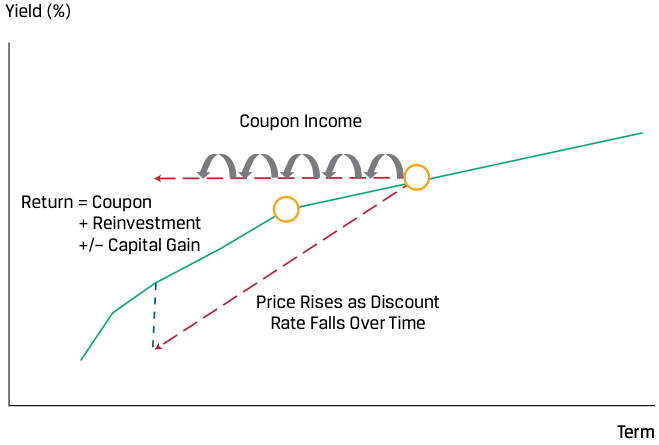
\includegraphics[scale=0.4]{/fi/yieldcurveroll}
\caption{Rolling down the yield curve}
\end{figure}

\begin{method} \hlt{Maturity Spread Carry Trade}\\
Borrowing at short-term rates and buying long maturity bonds, as short-term rates are very low, giving yield curves a steep upward slope.\\
The risk of the leveraged strategy is the possibility of an increase in spot prices.
\end{method}

\subsubsection{Short-Term Interest Rate Spreads}

\begin{definition} \hlt{Swap Spread}\\
Spread paid by the fixed-rate payer of an interest rate swap over the rate of the 'on-the-run' government security with the same maturity of the swap.\\
Captures yield premium required for credit relative to benchmark government bond, and is a barometer of the market's perceived credit risk relative to default-risk-free rates. Spread widens counter-cyclically.
\begin{equation}
\text{Swap Spread}_t = \text{Swap Rate}_t - \text{Treasury Yield}_t \nonumber
\end{equation}
\end{definition}

\begin{remark} \hlt{Usage of Swap Spread}\\
Swap rate are almost always positive, reflecting lower credit risk of governments compared to credit risk of surveyed banks that determines the swap rate.\\
Swap rate curve reflects default risk of a commercial bank with rating $A1/A+$.
\end{remark}

I-Spread and Z-Spread are referenced in the earlier subsection at Definition \ref{def:ispread} and Definition \ref{def:zpread}.

\begin{definition} \hlt{T-Bill Eurodollar Futures Contract Spread (TED Spread)}\\
Difference between MRR and the yield on a Treasury bill of the same maturity.
\begin{equation}
\text{TED Spread} = MRR - \text{T-Bill Rate} \nonumber
\end{equation}
As T-Bills are considered risk-free while MRR reflects risk of lending to commercial banks, TED Spread is an indicator of credit risk and liquidity risk in banking sector.\\
Increase in TED spread signals greater perceived credit and liquidity risk.
\end{definition}

\begin{figure}[H]
\centering
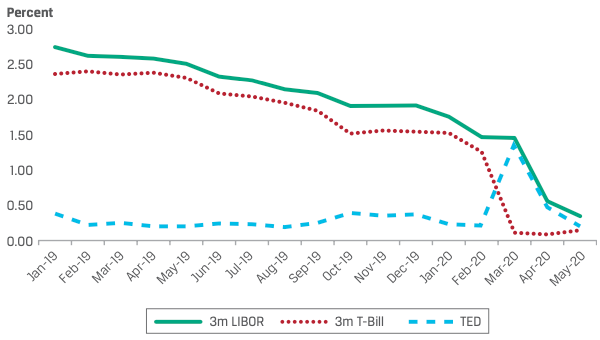
\includegraphics[scale=0.4]{/fi/tedspread}
\caption{T-Bill Eurodollar Futures Contract Spread}
\end{figure}

\begin{definition} \hlt{MRR-Overnight Indexed Swap Spread (MRR-OIS Spread)}\\
An OIS is an interest rate swap where periodic floating rate of the swap equals geometric average of a daily unsecured overnight rate (or overnight index rate).\\
The OIS rate roughly reflects the federal funds rate and includes minimal counterparty risk.\\
MRR-OIS Spread is the amount by which MRR exceeds OIS rate.\\
The spread indicates level of credit risk and liquidity risk in the banking system.
\end{definition}

\subsubsection{Term Structure Theory}

\begin{remark} \hlt{Unbiased/Pure Expectations Theory}\\
The hypothesis is that investor's expectations determine the shape of the interest rate term structure.\\
Forward rates are solely a function of expected future spot rates, and every maturity strategy has the same expected return over a given investment horizon.\\
Long-term interest rates equal the mean of future expected short-term rates.\\
Given an investment horizon, investor would be indifferent between investing in a single bond or splitting the investment into a sequence of bonds to hold.\\
Underlying principle is based on risk neutrality. Investors don't demand a risk premium for maturity strategies that differ from their investment horizon.
\end{remark}

\begin{remark} \hlt{Implications of Unbiased/Pure Expectations Theory}\\
The implications for the shape of yield curve under pure expectations theory are:
\begin{enumerate}[label=\roman*.]
\setlength{\itemsep}{0pt}
\item If yield curve is upward sloping, short-term rates are expected to rise
\item If yield curve is downward sloping, short-term rates are expected to fall
\item If yield curve is flat, short-term rates are expected to remain constant
\end{enumerate}
\end{remark}

\begin{remark} \hlt{Local Expectations Theory}\\
Similar to unbiased expectations theory, except that risk-neutrality assumption is only preserved for short holding periods. Over longer periods, risk premiums should exist.\\
Over short time periods, every bond (even long-maturity risky bonds) should earn risk-free rate.\\
Theory does not hold, as short-holding-period returns of long maturity bonds can be shown to be higher than short-holding-period returns of short maturity bonds due to liquidity premiums and hedging concerns.
\end{remark}

\begin{remark} \hlt{Liquidity Preference Theory}\\
Theory addresses shortcomings of pure expectations theory. Forward rates reflect investors' expectations of future spot rates, and liquidity premium compensates investors for exposure to interest rate risk.\\
Liquidity premium is positively related to maturity.\\
Forward rates are upwardly biased estimates of market's expectation of future rates due to inclusion of liquidity premium.\\
Positive-sloping yield curve indicates that either:
\begin{enumerate}[label=\roman*.]
\setlength{\itemsep}{0pt}
\item market expects future interest rates to rise, or
\item rates are expected to remain constant (or fall), but addition of liquidity premium results in positive slope.
\end{enumerate}
Downward-sloping yield curve indicates steeply falling short-term rates.\\
Size of liquidity premiums need not be constant over time; may be larger during periods of greater economic uncertainty when risk aversion among investors is higher.
\end{remark}

\begin{remark} \hlt{Segmented Markets Theory}\\
Theory allows for lender and borrower preferences to influence the shape of the yield curve, hence yields are not a reflection of expected spot rates or liquidity premiums, but rather is solely a function of supply and demand for funds of a particular maturity.\\
Yield at each maturity is determined independently of yields at other maturities.\\
Various market participants only deal in securities of a particular maturity as they are prevented from operating at different maturities (i.e., pension plans and insurance companies have asset-liability matching requirements).
\end{remark}

\begin{remark} \hlt{Preferred Habitat Theory}\\
Similar to segmented markets theory in that borrowers and lenders have strong preferences for particular maturities, but does not asset that yields at difference maturities are determined independently of each other.\\
If expected additional returns to be gained become large enough, investors will deviate from their preferred maturities or habitats, as investors will accept additional risk in return for additional expected returns. 
\end{remark}

\subsubsection{Yield Curve Factor Models}

\begin{definition} \hlt{Shaping Risk}\\
Sensitivity of bond price to changing shape of the yield curve.
\end{definition}

\begin{definition} \hlt{Three-Factor Model of Litterman and Scheinkman}\\
Yield curve risk may be decomposed into sensitivity to the following yield curve movements:
\begin{enumerate}[label=\roman*.]
\setlength{\itemsep}{0pt}
\item Level ($\Delta x_L$): a parallel increase or decrease of interest rates
\item Steepness ($\Delta x_S$): long-term interest rates increase while short-term interest rates decrease
\item Curvature ($\Delta x_C$): increase curvature means only short and long-term rates increase
\end{enumerate}
The model can then be implemented as
\begin{equation}
\frac{\Delta P}{P} = -D_L \Delta x_L - D_S \Delta x_S - D_C \Delta x_C \nonumber
\end{equation}
where $D_L, D_S, D_C$ are portfolio sensitivity to changes in yield curve's level, steepness, curvature.
\end{definition}

\begin{figure}[H]
\centering
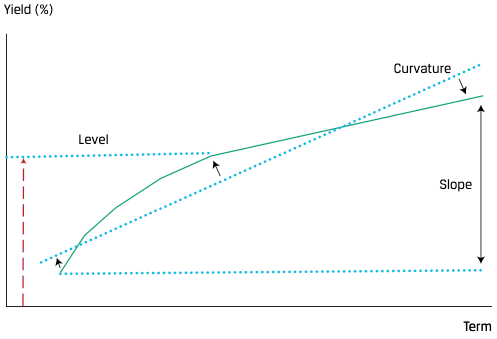
\includegraphics[scale=0.5]{/fi/yieldcurvefactor}
\caption{Yield curve factors: level, slope, curvature}
\end{figure}

\begin{remark} \hlt{Interest Rate Volatility} \\
Drives price volatility in a fixed income portfolio.\\
Important when securities have embedded options, which are especially sensitive to volatility.\\
Term structure of interest rate volatility is graph of yield volatility versus maturity.\\
Volatility at long-maturity end is associated with uncertainty on real economy and inflation.\\
Volatility at short-maturity end reflects risks regarding monetary policy.
\begin{equation}
\sigma(t,T) = \frac{\sigma[\Delta r(t,T)/r(t,T)]}{\sqrt{\Delta t}} \nonumber
\end{equation}
Uncertainty of an interest rate is measured by the annualised standard deviation of the proportional change in a bond yield over a specified interval.\\
Interest rate volatility measures annualised standard deviation of change in bond yield.
\end{remark}

\subsubsection{Interest Rate Views Using Macroeconomic Variables}

\begin{remark} \hlt{Macroeconomic Factors Effect on Bond Yields}\\
Macroeconomic factors that affect bond yields include inflation forecasts, GDP growth, monetary policy.\\
Two-thirds of variation in short- and intermediate-term yields is explained by monetary policy, rest by other factors. Inflation explains two-thirds of variation in long-term yields, remaining explained by monetary policy.
\end{remark}

\begin{definition} \hlt{Bond Risk Premium}\\
expected excess return of a default-free long-term bond less that of an equivalent short-term bond or the one-period risk-free rate. Measured using government bonds to capture uncertainty of default-free rates,
\end{definition}

\begin{remark} \hlt{Yield-Curve Flattening and Steepening}\\
In economic expansions, to combat rising inflation, central banks may raise short-term rates, leading to \hlt{bearish flattening} of the yield curve.\\
In recession, central banks may reduce short-term rates, leading to \hlt{bullish steepening}.
\end{remark}

\begin{figure}[H]
\centering
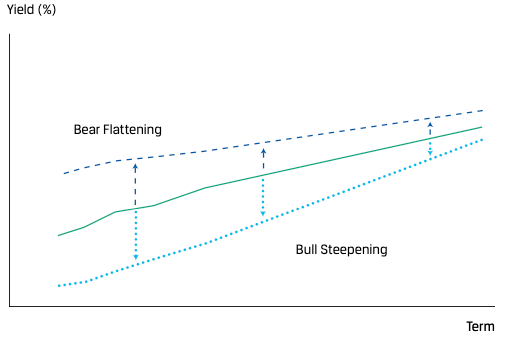
\includegraphics[scale=0.5]{/fi/yieldcurvesteep}
\caption{Yield curve flattening and steepening}
\end{figure}

\begin{remark} \hlt{Other Factors Affecting Bond Prices}
\begin{enumerate}[label=\roman*.]
\setlength{\itemsep}{0pt}
\item Fiscal policy: expansionary fiscal policies increase yields, vice versa
\item Maturity structure: government choice of maturity when issuing securities affect the supply and yield of bonds in those maturity segments. Increase in offerings in specific segment of the market increases the supply and the yield in the segment (by market segmentation theory)
\item Investor demand: pension and insurance firms prefer longer maturity bonds, driving down long-term yields. In high uncertainty markets, flight to safety may reduce long-term government bond yields, resulting in bullish flattening of the yield curve.
\end{enumerate}
\end{remark}

\begin{remark} \hlt{Investor Actions}\\
In expectation of rise (fall) in rates, investors will lower (extend) duration of their bond portfolios.\\
Expectation of steepening of yield curve may lead investors to long short-term bonds, short long-term bonds.\\
Trades may be designed to be duration-neutral so change in level of interest rates does not affect value of the portfolio. Investors with long-only mandates may rotate between bullet portfolio (portfolio concentrated in a single maturity) and a barbell portfolio (portfolio with short and long maturities).\\
Expectation of bullish flattening of yield curve may lead investor to rotate out of bullet into barbell portfolio.
\end{remark}